\chapter{Conversione Digitale--Analogica e Analogica--Digitale}
\label{ch:dac}
\textit{(15 maggio 2026)}

% ======================================================================
\section{Conversione digitale $\leftrightarrow$ analogica}

Le grandezze fisiche (temperatura, pressione, suono, \ldots) sono analogiche, mentre la loro
elaborazione avviene quasi sempre in digitale. Un sistema di acquisizione, come l'Analog
Discovery 2 (AD2) usato in laboratorio, trasforma quindi la tensione fornita da un sensore in
una sequenza di numeri e, se serve, ricostruisce poi un segnale analogico:

\begin{fitcenter}
\begin{tikzpicture}[font=\small, >=latex, line width=0.6pt,
  blocco/.style={draw, thick, minimum width=1.6cm, minimum height=0.9cm, align=center, fill=noteblue!4}]
% segnale campionato
\draw[->] (0,0) -- (3.2,0) node[right] {$t$};
\draw[->] (0,0) -- (0,2.0) node[above] {$V$};
\foreach \x/\y in {0.4/1.2, 0.8/0.8, 1.2/0.6, 1.6/0.9, 2.0/1.3, 2.4/1.6, 2.8/1.5}{
  \node[font=\footnotesize, text=noteblue] at (\x,\y) {$\times$};
}
\node[font=\scriptsize] at (1.6,2.75) {campionamenti $V(t_i)$};
% blocchi
\node[blocco] (sen) at (4.8,1.0) {Sensore};
\node[blocco] (adc) at (7.4,1.0) {ADC\\\scriptsize(es. AD2)};
\node[blocco] (el)  at (10.2,1.0) {elaborazione\\digitale};
\node[blocco] (dac) at (13.0,1.0) {DAC};
\draw[->, thick] (sen) -- node[above, font=\scriptsize] {$V_{\text{in}}$} (adc);
\draw[->, thick] (adc) -- node[above, font=\scriptsize] {$n_{\text{out}}$} (el);
\draw[->, thick] (el) -- node[above, font=\scriptsize] {$n_{\text{in}}$} (dac);
% segnale ricostruito
\begin{scope}[xshift=14.6cm]
\draw[->] (0,0) -- (3.2,0) node[right] {$t$};
\draw[->] (0,0) -- (0,2.0) node[above] {$V$};
\draw[thick, noteblue] (0.4,1.2) -- (0.8,0.8) -- (1.2,0.6) -- (1.6,0.9) -- (2.0,1.3) -- (2.4,1.6) -- (2.8,1.5);
\foreach \x/\y in {0.4/1.2, 0.8/0.8, 1.2/0.6, 1.6/0.9, 2.0/1.3, 2.4/1.6, 2.8/1.5}{
  \node[font=\footnotesize, text=noteblue] at (\x,\y) {$\times$};
}
\node[font=\scriptsize, align=center] at (1.8,2.9) {ricostruzione (interpolazione lineare)};
\end{scope}
\draw[->, thick] (dac.east) -- (14.5,1.0);
\end{tikzpicture}
\end{fitcenter}

\noindent Che cosa succede fra il sensore e il segnale ricostruito? La catena è:
\begin{align*}
&\text{\textbf{sample and hold}} \;\longrightarrow\; \text{\textbf{convertitore analogico--digitale (ADC)}} \;\longrightarrow\\
&\longrightarrow\; \text{elaborazione digitale} \;\longrightarrow\; \text{\textbf{convertitore digitale--analogico (DAC)}}
\end{align*}
Il \emph{sample and hold} preleva il valore della tensione in un istante $t_i$ e lo mantiene
costante per tutto il tempo necessario alla conversione; l'ADC lo trasforma in un numero;
dopo l'elaborazione il DAC riporta i numeri in tensioni, che vengono raccordate
(nel caso più semplice con segmenti di retta).

\medskip
\noindent Definizioni di base, per un convertitore a $N$ bit:
\begin{itemize}[leftmargin=1.5em, itemsep=2pt]
    \item $n$ = numero intero che dipende dai bit disponibili: $0 \le n \le 2^N-1$;
    \item $\Delta V$ = \textbf{granularità}, cioè il passo minimo distinguibile (la tensione
          che corrisponde a 1 LSB);
    \item $V_{\text{ref}}$ = tensione di riferimento, cioè il \textbf{valore massimo
          ottenibile} (il fondo scala). Non va confusa con $\Delta V$: i due sono legati da
          \[
          \Delta V = \frac{V_{\text{ref}}}{2^N}
          \]
\end{itemize}

\begin{definizione}{Funzioni di trasferimento}
\textbf{ADC}: \quad $n_{\text{out}} = \dfrac{V_{\text{in}}}{\Delta V}$ \quad (arrotondato a un
numero intero)\\[0.6em]
\textbf{DAC}: \quad $V_{\text{out}} = n_{\text{in}} \cdot \Delta V$
\end{definizione}

% ======================================================================
\section{Caratteristiche del DAC}

\begin{definizione}{Precisione}
determinata dal numero di bit e dall'intervallo di tensioni: $V_{\text{out}} = n_{\text{in}}\,\Delta V$.
\end{definizione}

\noindent Ad esempio, con $N=3$ bit e $\Delta V = 1\,\text{V}$:
$n_{\text{in}} \in [0,\, 2^3-1] = [0,7] \;\Rightarrow\; V_{\text{out}} \in [0,\,7]\,\text{V}$,
con passi da 1\,V. A parità di intervallo, aumentare il numero di bit riduce $\Delta V$ e
rende l'uscita più fine.

\medskip
\noindent La \textbf{velocità di conversione} è molto importante e dipende da vari fattori:
il \textbf{tempo di assestamento} dell'uscita dopo un cambio del codice, l'\textbf{architettura}
del convertitore e il \textbf{numero di bit} (più bit, in genere, significano una
conversione più lenta).

\medskip
\noindent Il comportamento reale di un DAC si discosta da quello ideale per tre principali
sorgenti di errore:

\begin{center}
\begin{minipage}[t]{0.32\linewidth}\centering
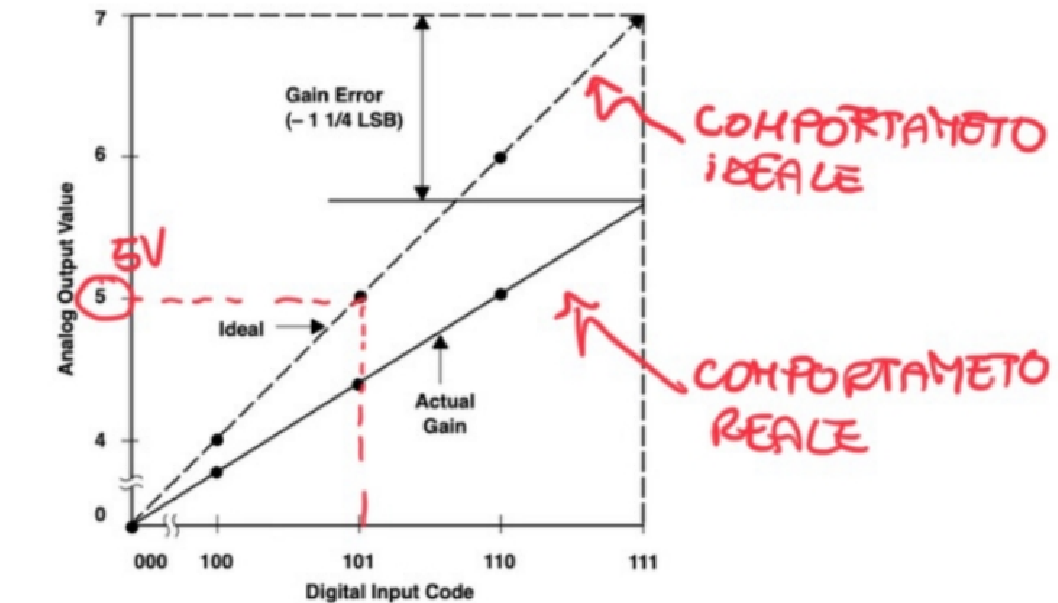
\includegraphics[width=\linewidth]{err_g.png}\\
\footnotesize (a) errore di guadagno
\end{minipage}\hfill
\begin{minipage}[t]{0.32\linewidth}\centering
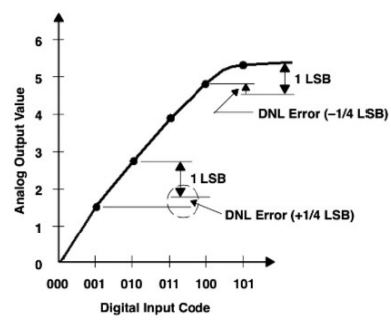
\includegraphics[width=\linewidth]{n_lin.png}\\
\footnotesize (b) non linearità
\end{minipage}\hfill
\begin{minipage}[t]{0.32\linewidth}\centering
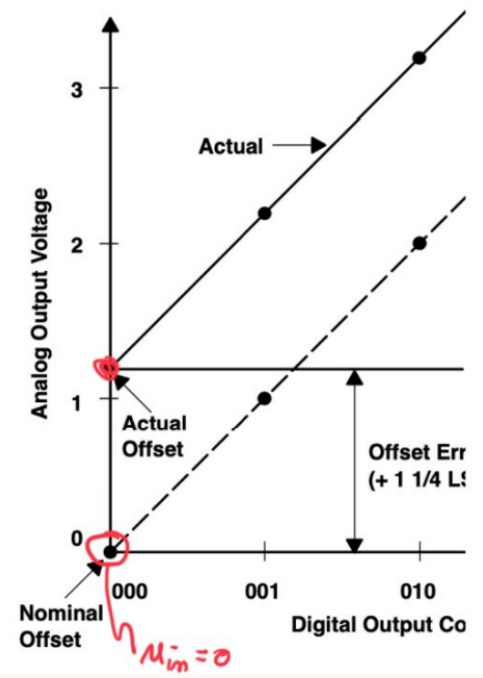
\includegraphics[width=\linewidth]{er_nlin.png}\\
\footnotesize (c) errore di offset
\end{minipage}
\end{center}

\begin{itemize}[leftmargin=1.5em, itemsep=2pt]
    \item \textbf{(a) Errore di guadagno}: la caratteristica reale è una retta con pendenza
          diversa da quella ideale; l'errore cresce con il codice ed è massimo a fondo scala.
    \item \textbf{(b) Non linearità}: i gradini non sono tutti uguali, per cui la
          caratteristica si incurva. La non linearità differenziale (DNL) misura quanto ogni
          singolo passo differisce da 1 LSB.
    \item \textbf{(c) Errore di offset}: la caratteristica è traslata; per $n_{\text{in}}=0$
          l'uscita non vale 0 e l'errore è lo stesso per tutti i codici.
\end{itemize}

% ======================================================================
\section{DAC a sommatore}

L'architettura più semplice di DAC è il \textbf{DAC a sommatore pesato}: un amplificatore
operazionale in configurazione invertente somma le correnti di più resistenze di ingresso,
una per bit. Ogni resistenza è collegata a $V_{\text{ref}}$ se il bit vale $a_i=1$ oppure a
massa se $a_i=0$, tramite uno \textbf{switch} comandato dal bit.

\begin{fitcenter}
\begin{circuitikz}[line width=0.6pt, font=\small, american]
\node[op amp, anchor=-] (OA) at (6.2,1.4) {};
\draw (OA.+) -- ++(-0.4,0) node[ground] {};
\coordinate (S) at (5.2,1.4);
\draw (S) -- (OA.-);
\draw (S) -- (S |- 0,-1.4);
\draw (S) -- (S |- 0,3.0) to[R, l=$R$] (OA.out |- 0,3.0) -- (OA.out);
\draw (OA.out) to[short, -o] ++(0.8,0) node[right] {$V_{\text{out}}$};
\foreach \i/\y/\r/\lab in {2/1.4/{R/4}/MSB, 1/0/{R/2}/, 0/-1.4/R/LSB}{
  \draw (S |- 0,\y) node[circle, fill, inner sep=1pt] {} to[R, l=$\r$] (1.6,\y) coordinate (P\i);
  \draw (P\i) node[circle, fill, inner sep=1pt] {} -- (0.9,\y+0.3);
  \draw (0.8,\y+0.4) node[circle, draw, fill=white, inner sep=1pt] {} -- (0.2,\y+0.4) node[left, font=\scriptsize] {$V_{\text{ref}}$};
  \draw (0.8,\y-0.4) node[circle, draw, fill=white, inner sep=1pt] {} -- (0.2,\y-0.4) node[ground, scale=0.6] {};
  \node[font=\scriptsize, color=noteblue, anchor=north west] at (1.1,\y-0.05) {$a_\i$};
  \node[font=\scriptsize, color=noteblue, anchor=east] at (-0.6,\y) {\lab};
}
\end{circuitikz}
\end{fitcenter}

\noindent Poiché l'ingresso invertente è una massa virtuale, ogni ramo porta una corrente
indipendente dagli altri, $I_i = a_i V_{\text{ref}}/R_i$, e tutte le correnti attraversano la
resistenza di retroazione $R$. Per sovrapposizione degli effetti (qui con tutti i bit a 1):
\[
V_{\text{out}} = -V_{\text{ref}}\left(\frac{R}{R_0}+\frac{R}{R_1}+\frac{R}{R_2}\right)
\]
Scegliendo resistenze pesate $R_i = R/2^i$ si ha $R/R_i = 2^i$ e quindi
$V_{\text{out}} = -V_{\text{ref}}\sum_i 2^i$. Considerando gli switch, ogni bit vale
$a_i=0$ (collegamento a massa) oppure $a_i=1$ (collegamento a $V_{\text{ref}}$):
\[
\boxed{V_{\text{out}} = -V_{\text{ref}}\sum_{i=0}^{N-1} a_i\,2^i}
\]
Il bit più significativo ha la resistenza più piccola ($R/2^{N-1}$) e quindi il peso
maggiore. Con 3 bit e ingresso $101_2$: $V_{\text{out}} = -V_{\text{ref}}(4+1) = -5\,V_{\text{ref}}$.

\begin{important}
\textbf{Limite pratico.} Supponiamo di avere 10 bit con $R_i = 100\,\text{k}\Omega/2^i$: le
resistenze vanno da $100\,\text{k}\Omega$ (LSB) a circa $98\,\Omega$ (MSB).
\begin{itemize}[leftmargin=1.3em, itemsep=2pt]
    \item Se la tolleranza vale $\sigma_0 = 1\%$ di $R_0 = 100\,\text{k}\Omega$, cioè
          $\sigma_0 = 1\,\text{k}\Omega$, e l'incertezza assoluta è la stessa per tutte le
          resistenze, quelle dei bit più pesanti sono addirittura più piccole
          dell'incertezza ($R_i < \sigma_0$ per $i \ge 7$: $R_7 \approx 781\,\Omega$).
    \item Anche con una tolleranza relativa dell'1\% su ogni resistenza, il bit più
          significativo pesa $2^9=512$ volte l'LSB e il suo errore vale circa $5$ LSB, molto
          più del contributo dei bit meno significativi. Questi bit vengono quindi
          \textbf{persi}: per non perderli servirebbe una tolleranza inferiore a
          $1/2^N$ (circa $0{,}1\%$ per 10 bit).
    \item Resistenze con valori così diversi sono difficili da realizzare con la stessa
          precisione, soprattutto in un circuito integrato.
\end{itemize}
Il DAC a sommatore si può quindi usare solo se abbiamo pochi bit, altrimenti non è utile.
\end{important}

% ======================================================================
\section{DAC R-2R Ladder}

Per avere un DAC più preciso si usa la tecnica \textbf{R-2R Ladder} (rete a scala), che
genera pesi binari per i bit usando \textbf{solo due valori di resistenza}, $R$ e $2R$.
È molto più facile ottenere resistenze tutte uguali (e con errori correlati) che resistenze
di valori molto diversi.

\begin{fitcenter}
\begin{circuitikz}[line width=0.6pt, font=\small, american]
% nodi della scala: MSB in alto
\foreach \i/\y in {0/4.5, 1/3.0, 2/1.5, 3/0}{
  \coordinate (N\i) at (4,\y);
  \draw (N\i) node[circle, fill, inner sep=1.2pt] {} to[R, l_=$2R$] (1.6,\y) coordinate (P\i);
  \draw (P\i) node[circle, fill, inner sep=1pt] {} -- (0.9,\y+0.3);
  \draw (0.8,\y+0.4) node[circle, draw, fill=white, inner sep=1pt] {} -- (0.2,\y+0.4) node[left, font=\scriptsize] {$V_{\text{ref}}$};
  \draw (0.8,\y-0.4) node[circle, draw, fill=white, inner sep=1pt] {} -- (0.2,\y-0.4) node[ground, scale=0.6] {};
  \node[font=\scriptsize, color=noteblue, anchor=north west] at (1.1,\y-0.05) {$a_\i$};
}
\draw (N0) to[R, l=$R$] (N1) to[R, l=$R$] (N2) to[R, l=$R$] (N3);
\draw (N3) to[R, l=$2R$] (4,-1.6) node[ground] {};
\node[font=\scriptsize, color=noteblue, anchor=east] at (-0.6,4.5) {MSB};
\node[font=\scriptsize, color=noteblue, anchor=east] at (-0.6,0) {LSB};
% amplificatore
\node[op amp, anchor=-] (OA) at (6.6,4.5) {};
\draw (N0) -- (OA.-);
\draw (OA.+) -- ++(-0.4,0) node[ground] {};
\draw (5.6,0 |- OA.-) node[circle, fill, inner sep=1.2pt] {} -- (5.6,5.8) to[R, l=$R$] (OA.out |- 0,5.8) -- (OA.out);
\draw (OA.out) to[short, -o] ++(0.8,0) node[right] {$V_{\text{out}}$};
\end{circuitikz}
\end{fitcenter}

\noindent\textbf{Perché i pesi sono binari.} Guardando verso il basso da un qualsiasi nodo, la
parte di scala sottostante ha resistenza equivalente $2R$ (partendo dal fondo:
$2R \parallel 2R = R$, in serie a $R$ dà di nuovo $2R$, e così via). A ogni nodo, quindi, il
contributo di tensione di un bit viene diviso per 2 salendo di un gradino. Ne segue che il
bit $a_i$ ($i=0$ MSB) contribuisce all'uscita con
\[
a_i \;\longrightarrow\; V_{\text{out},i} = -\frac{V_{\text{ref}}}{2^{i+1}}
\qquad\Rightarrow\qquad \text{i pesi sono } \frac{1}{2},\,\frac{1}{4},\,\frac{1}{8},\,\frac{1}{16},\,\ldots
\]
e sommando tutti i contributi:
\[
\boxed{V_{\text{out}} = -V_{\text{ref}}\sum_{i=0}^{N-1} \frac{a_i}{2^{i+1}}}
\]
L'uscita massima (tutti i bit a 1) vale $-V_{\text{ref}}(1-2^{-N})$, cioè il fondo scala meno
un LSB, e il passo è $\Delta V = V_{\text{ref}}/2^N$.

\begin{esercizio}{Esempio}
Con 4 bit, ingresso $a_0a_1a_2a_3 = 1010$ e $V_{\text{ref}} = 8\,\text{V}$:
\[
V_{\text{out}} = -8\left(\frac{1}{2}+\frac{1}{8}\right) = -8 \cdot \frac{5}{8} = -5\,\text{V}
\]
In modulo il risultato coincide con $n_{\text{in}}\,\Delta V = 10 \cdot \frac{8}{16} = 5\,\text{V}$.
\end{esercizio}

\begin{osservazione}{Scelta delle resistenze di terminazione e di retroazione}
Negli appunti la terminazione in fondo alla scala è indicata come $R$ e la resistenza di
retroazione come $2R$. Risolvendo il circuito (nodo MSB a massa virtuale) con le quattro
combinazioni possibili si ottiene, per l'esempio $1010$ con $V_{\text{ref}}=8$\,V:
\begin{center}
\small\renewcommand{\arraystretch}{1.6}
\begin{tabular}{c|c|c|c}
\toprule
terminazione & retroazione & pesi dei bit $a_0,a_1,a_2,a_3$ & $V_{\text{out}}(1010)$ \\
\midrule
$R$  & $2R$ & $1,\ \tfrac{42}{85},\ \tfrac{4}{17},\ \tfrac{8}{85}$ & $-9{,}88$\,V \\
$R$  & $R$  & $\tfrac12,\ \tfrac{21}{85},\ \tfrac{2}{17},\ \tfrac{4}{85}$ & $-4{,}94$\,V \\
$2R$ & $2R$ & $1,\ \tfrac12,\ \tfrac14,\ \tfrac18$ & $-10$\,V \\
$\mathbf{2R}$ & $\mathbf{R}$ & $\tfrac12,\ \tfrac14,\ \tfrac18,\ \tfrac1{16}$ & $\mathbf{-5}$\,\textbf{V} \\
\bottomrule
\end{tabular}
\end{center}
\begin{itemize}[leftmargin=1.3em, itemsep=1pt]
    \item Con terminazione $R$ i pesi \textbf{non sono più potenze di 2}: la scala vede
          verso il basso una resistenza diversa da $2R$ e la divisione per 2 a ogni nodo
          non vale più. La terminazione deve quindi essere $2R$.
    \item La retroazione fissa solo il guadagno: con $2R$ tutte le uscite raddoppiano.
          Il risultato degli appunti ($5$\,V, cioè pesi $\tfrac12,\tfrac14,\ldots$) si
          ottiene solo con retroazione $R$, uguale alla resistenza equivalente della scala.
\end{itemize}
Lo schema e le formule di questa sezione usano quindi terminazione $2R$ e retroazione $R$.
\end{osservazione}

% ======================================================================
\section{Caratteristiche dell'ADC}

\begin{itemize}[leftmargin=1.5em, itemsep=2pt]
    \item \textbf{Accuratezza}: insieme di tutte le sorgenti di errore; comprende sempre
          almeno l'errore di quantizzazione.
    \item \textbf{Errore di quantizzazione}: dipende dal tipo di ADC ed è dovuto alla
          discretizzazione del segnale durante la conversione. Tutte le tensioni che cadono
          nello stesso gradino producono lo stesso codice, quindi l'informazione all'interno
          di un gradino è persa. Di solito vale $1$ LSB (se il codice è ottenuto per
          troncamento) oppure $\pm 0{,}5$ LSB (se i gradini sono centrati sui valori ideali).
    \item \textbf{Tempo di conversione} e \textbf{principio di funzionamento} sono le altre
          caratteristiche importanti (i diversi tipi di ADC sono trattati nel capitolo
          successivo).
\end{itemize}

\begin{center}
\begin{tikzpicture}[x=0.75cm, y=0.55cm, font=\scriptsize, line width=0.6pt, >=latex]
\draw[->] (0,0) -- (8.6,0) node[right] {$V_{\text{in}}/\Delta V$};
\draw[->] (0,0) -- (0,8) node[above] {$n_{\text{out}}$};
\draw[dashed, gray] (0,0) -- (8,8);
\draw[thick, noteblue] (0,0) \foreach \k in {0,...,6}{ -- (\k+0.5,\k) -- (\k+0.5,\k+1) } -- (8,7);
\foreach \k in {0,...,7}{ \node[left] at (0,\k) {\k}; }
\foreach \k in {0,...,8}{ \node[below] at (\k,0) {\k}; }
\begin{scope}[yshift=-2.6cm]
\draw[->] (0,0) -- (8.6,0) node[right] {$V_{\text{in}}/\Delta V$};
\draw[->] (0,-1.2) -- (0,1.4) node[above] {errore};
\draw[thick, notered] (0,0) \foreach \k in {0,...,6}{ -- (\k+0.5,-0.5*1.6) -- (\k+0.5,0.5*1.6) } -- (7.5,-0.8);
\node[left] at (0,0.8) {$+\frac{1}{2}$ LSB};
\node[left] at (0,-0.8) {$-\frac{1}{2}$ LSB};
\end{scope}
\end{tikzpicture}
\end{center}

\noindent Nella figura (ADC ideale a 3 bit con gradini centrati) la caratteristica a gradini
approssima la retta ideale tratteggiata; la differenza fra le due è l'errore di
quantizzazione, un ``dente di sega'' compreso fra $-\frac12$ e $+\frac12$ LSB.

\medskip
\noindent Analogamente al DAC, anche l'ADC presenta tre principali tipi di errore rispetto
al comportamento ideale (linea tratteggiata = ADC ideale, linea continua = ADC reale):

\begin{center}
\begin{minipage}[t]{0.32\linewidth}\centering
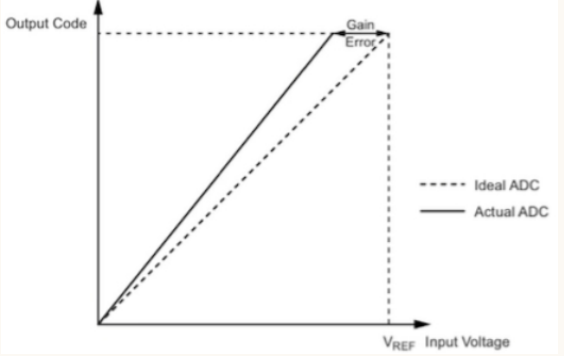
\includegraphics[width=\linewidth]{err_g2.png}\\
\footnotesize (a) errore di guadagno
\end{minipage}\hfill
\begin{minipage}[t]{0.32\linewidth}\centering
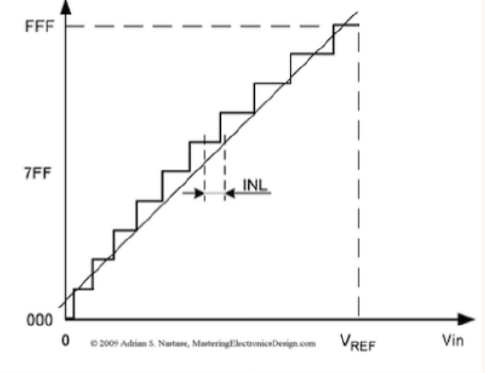
\includegraphics[width=\linewidth]{n_lin2.png}\\
\footnotesize (b) non linearità integrale (INL)
\end{minipage}\hfill
\begin{minipage}[t]{0.32\linewidth}\centering
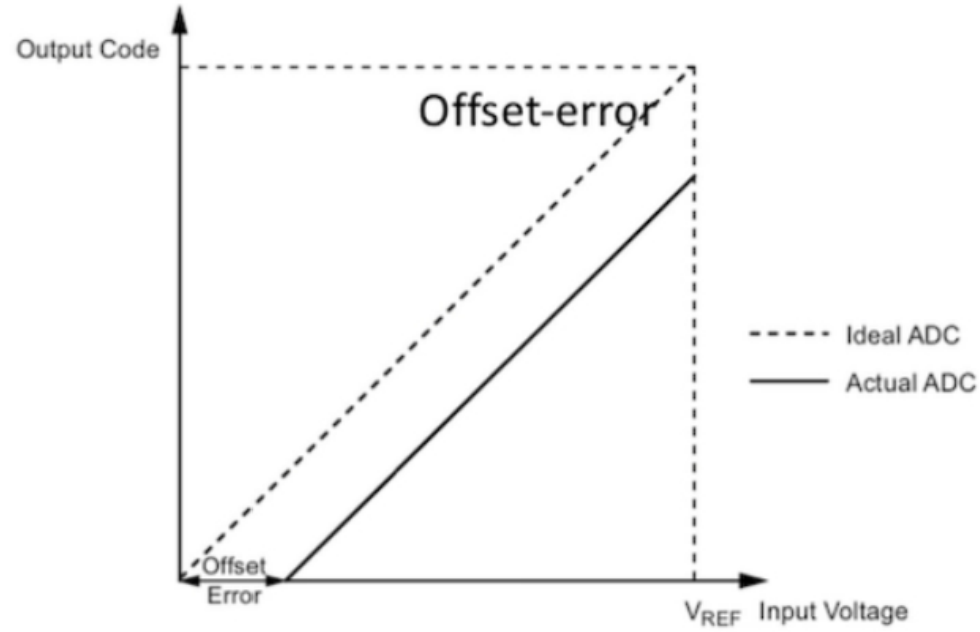
\includegraphics[width=\linewidth]{er_nlin2.png}\\
\footnotesize (c) errore di offset
\end{minipage}
\end{center}

\begin{itemize}[leftmargin=1.5em, itemsep=2pt]
    \item \textbf{(a) Errore di guadagno}: la pendenza della caratteristica reale è diversa da
          quella ideale, per cui il codice massimo viene raggiunto a una tensione diversa da
          $V_{\text{ref}}$.
    \item \textbf{(b) Non linearità integrale (INL)}: massima distanza fra la caratteristica a
          gradini reale e la retta ideale, lungo tutto l'intervallo di ingresso.
    \item \textbf{(c) Errore di offset}: la caratteristica è traslata, per cui la prima
          transizione avviene a una tensione diversa da quella ideale.
\end{itemize}

% ======================================================================
\section*{Riepilogo del Capitolo}

\begin{important}
La conversione Digitale-Analogica è caratterizzata dalla risoluzione $\Delta V = V_{\text{ref}}/2^N$; il DAC a sommatore pesato è concettualmente semplice ma impraticabile con molti bit per i vincoli di tolleranza sulle resistenze, superati dal \textbf{DAC R-2R Ladder}, che usa soltanto due valori di resistenza.
\end{important}

\begin{note}
\textbf{Formule fondamentali:}
\begin{itemize}
    \item \textbf{Risoluzione (granularità):} $\Delta V = V_{\text{ref}}/2^N$.
    \item \textbf{DAC a sommatore pesato:} $V_{\text{out}} = -V_{\text{ref}} \sum_{i=0}^{N-1} a_i\, 2^i$, con $R_i = R/2^i$.
    \item \textbf{DAC R-2R Ladder:} $V_{\text{out}} = -V_{\text{ref}} \sum_{i=0}^{N-1} \dfrac{a_i}{2^{i+1}}$.
    \item \textbf{Errori caratteristici:} di guadagno, di offset e di non linearità differenziale (DNL).
\end{itemize}
\end{note}

